% Copyright (c)  2005-2010 EDF-EADS-PHIMECA.
% Permission is granted to copy, distribute and/or modify this document
% under the terms of the GNU Free Documentation License, Version 1.2
% or any later version published by the Free Software Foundation;
% with no Invariant Sections, no Front-Cover Texts, and no Back-Cover
% Texts.  A copy of the license is included in the section entitled "GNU
% Free Documentation License".
\renewcommand{\etapemethodo}{Resp. Surf.}
\renewcommand{\nomfichier}{docref_SurfRep_PCTrunc}
\renewcommand{\titrefiche}{Truncation schemes for the polynomial chaos expansion}

%\newcommand{\mathA}{\mathcal{A}}

\Header

\MathematicalDescription{
\underline{\textbf{Goal}} \vspace{4mm}

The polynomial chaos (PC) expansion allows one to obtain an explicit representation of the random response $\underline{Y}$ of the model under consideration, see~\otref{docref_SurfRep_PCBasis}{PC basis}. More precisely, the response $Y$ is cast as a converging series featuring orthonormal polynomials. For computational purpose, it is necessary though to retain a finite number of terms by truncating the expansion. Strategies for enumerating the infinite PC basis have been introduced \otref{docref_SurfRep_Enum}{Strategies for enumerating the polynomial chaos basis}. Then it is possible to device several strategies in order to truncate the representation, as shown in the sequel.\\

\underline{\textbf{Principle}} \vspace{4mm}

As shown in~\otref{docref_SurfRep_PCBasis}{PC basis}, the random model response $\underline{Y}$ may be expanded onto the PC basis as follows:
\begin{equation} 
    \underline{Y} \, \,  = \, \,  h(\underline{X}) \, \, = \, \, \sum_{\idx \in \mathbb{N}^{n_X}} \; \underline{a}_{\idx} \; \psi_{\idx}(\underline{X})
\end{equation}
where $n$ denotes the dimension of vector $\bs{X}$. For practical implementation, \emph{finite dimensional} polynomial chaoses have to be built. In other words, a suitable finite subset $\mathA$ of $\mathbb{N}^{n_X}$ has to be selected. Using a specific enumeration strategy, a one-to-one mapping between natural integers $j$ and the multi-indices $\idx$ in $\mathbb{N}^{n_X}$ is created and the PC series rewrites:
\begin{equation} 
    \underline{Y} \, \,  = \, \,  h(\underline{X}) \, \, = \, \, \sum_{j=0}^{\infty} \; \underline{a}_{j} \; \psi_{j}(\underline{X})
\end{equation}

\paragraph*{Fixed strategy\\}

The so-called \emph{fixed strategy} simply consists in retaining the first $P$ elements of the PC basis, the latter being ordered according to a given enumeration scheme (hyperbolic or not). The retained set is built \emph{in a single pass}. The truncated PC expansion is given by:
\begin{equation} 
    \widehat{h}(\underline{X}) \, \, = \, \, \sum_{j=0}^{P-1} \; \underline{a}_{j} \; \psi_{j}(\underline{X})
\end{equation}
In case of a linear enumeration strategy, a usual choice is to set $P$ equal to $\binom{n_X+p}{p} = \frac{(n_X+p)!}{n_X!p!}$, for a given natural integer $p$. This way the set of retained basis functions $\{\psi_{j},j=0,\dots,P-1\}$ gathers all the polynomials with total degree not greater than $p$. The number of terms $P$ grows polynomially both in $n_X$ and $p$ though, which may lead to difficulties in terms of computational efficiency and memory requirements when dealing with high-dimensional problems. 

\paragraph*{Sequential strategy\\}

The \emph{sequential strategy} consists in constructing the basis of the truncated PC \emph{iteratively}. Precisely, one begins with the first term $\psi_0$, that is $\mathA_{0} = \{0\}$, and one complements the current basis as follows: $\mathA_{k+1} = \mathA_{k} \cup \{\psi_{k+1}\}$. The construction process is stopped when a given accuracy criterion is reached, or when $P$ is equal to a prescribed maximum basis size $P_{max}$.

\paragraph*{Cleaning strategy\\}

The \emph{cleaning strategy} is aimed at building a PC expansion containing at most $P$ significant coefficients, i.e. at most $P$ significant basis functions. It proceeds as follows:
\begin{itemize}
\item Generate an initial PC basis made of the $P$ first polynomials (according to the adopted enumeration strategy), or equivalently an initial set of indices $\mathA = \{0,\dots,P-1\}$
 \item Discard from the basis all those polynomials $\psi_j$ associated with insignificant coefficients, i.e. the coefficients that satisfy:
 \begin{equation} 
    |a_j| \, \, \leq \, \, \varepsilon \; \cdot \; \max_{k \in \mathA} |a_k| 
\end{equation}
where $\varepsilon$ is a given tolerance, e.g. $\varepsilon = 10^{-4}$.
\item Add the next basis term $\psi_{P}$ to the current basis $\mathA$
\item Reiterate the procedure until either $P$ terms have been retained or if a given number $P_{max}$ of candidate terms have been considered 
\end{itemize} 

% The usual choice consists in selecting those multivariate polynomials $\psi_{\idx}$ of total degree $\|\idx \|_{1} \equiv \sum_{i=1}^{n} \alpha_i$ not greater than a maximal degree $p$, that is:
% \begin{equation} 
%     \underline{Y} \, \, \, \approx \, \, \, h_p(\underline{X})  \, \,  = \, \, \sum_{\|\idx \|_{1} \leq p} \; \underline{a}_{\idx} \; \psi_{\idx}(\underline{X})
% \end{equation}
% The corresponding \emph{truncation set} is defined by:
% \begin{equation} 
% 	\mathA^{n,p} \, \, \equiv \, \, \left\{\idx \in \Nn \, : \, \|\idx \|_{1}  \leq p \right\}
% \end{equation} 
% The size of the resulting finite-dimensional basis is denoted by $P$ and given by:
% \begin{equation}
% 	P \, \, = \, \, \binom{n+p}{p} \, \, = \, \, \frac{(n+p)!}{n!p!}
% \end{equation}
% hence a number of terms that grows polynomially both with $p$ and $n$. This may lead to intractable calculations in high dimensions (say $n\geq 10$) since the number $N$ of model evaluations increases with $P$. To overcome this difficulty, an alternative strategy for truncating the PC expansion is considered, namely the \emph{hyperbolic} scheme.  \\
% 
% The hyperbolic truncation strategy is inspired by the so-called \emph{sparsity-of-effects principle}, which states that most models are principally governed by main effects and low-order interactions. One proposes the use of the following truncation sets based on $q$-quasi-norms, $0<q<1$:
% \begin{equation} \label{eq:4.2:14}
% 	  \mathA^{n,p}_{q} \, \, \equiv \, \,  \{\idx \in \Nn \, : \, \| \idx \|_{q} \leq p \}
% \end{equation}  
% where:
% \begin{equation} \label{eq:4.2:15}
% 	 \| \idx \|_{q} \, \, \equiv \, \, \left(\sum_{i=1}^{n} \alpha_{i}^{q}\right)^{1/q} 
% \end{equation}  
% Such norms penalize the indices associated with high-order interactions all the more since $q$ is low. This phenomenon is depicted in the figures below for $n=2$, where the retained PC basis monomials are represented for various values of $p$ and $q$.
% 
% \begin{center}		\includegraphics[width = 9cm]{qnorms_2D_princ.pdf} \end{center}
% \begin{center}	 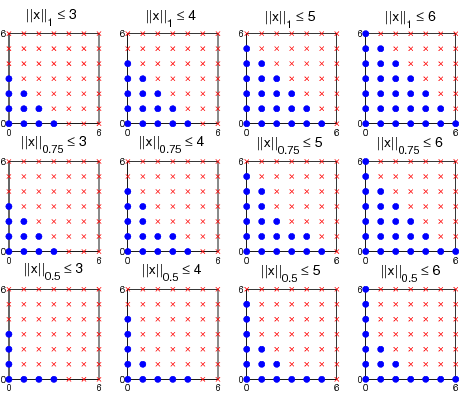
\includegraphics[width = 8cm]{qnorms_2D.pdf} \end{center}
% 
% Note that setting $q$ equal to 1 corresponds to the usual truncation scheme, i.e. $\mathA^{M,p}_{1} = \mathA^{M,p}$. When using $q < 1$, the retained basis polynomials are located under an hyperbola, hence the name \emph{hyperbolic truncation scheme}.
 

}

{
  --
}

\Methodology{
Within the global methodology, the polynomial chaos expansion of the model under consideration is built up prior to tackling the step C: ``Uncertainty propagation''. Then the various uncertainty propagation techniques may be applied at a negligible computational cost. The method requires to have fulfilled the two following steps:
\begin{itemize}
  \item step A1: identify of an input vector $\vect{X}$ of sources of uncertainties and an output variable of interest $\underline{Y} = h(\underline{X})$;
  \item step B: identify one of the proposed techniques to estimate a probabilistic model of the input vector $\vect{X}$.
  \end{itemize}
}
{

}


